%%
%% This is file `sample-authordraft.tex',
%% generated with the docstrip utility.
%%
%% The original source files were:
%%
%% samples.dtx  (with options: `authordraft')
%% 
%% IMPORTANT NOTICE:
%% 
%% For the copyright see the source file.
%% 
%% Any modified versions of this file must be renamed
%% with new filenames distinct from sample-authordraft.tex.
%% 
%% For distribution of the original source see the terms
%% for copying and modification in the file samples.dtx.
%% 
%% This generated file may be distributed as long as the
%% original source files, as listed above, are part of the
%% same distribution. (The sources need not necessarily be
%% in the same archive or directory.)
%%
%% Commands for TeXCount
%TC:macro \cite [option:text,text]
%TC:macro \citep [option:text,text]
%TC:macro \citet [option:text,text]
%TC:envir table 0 1
%TC:envir table* 0 1
%TC:envir tabular [ignore] word
%TC:envir displaymath 0 word
%TC:envir math 0 word
%TC:envir comment 0 0
%%
%%
%% The first command in your LaTeX source must be the \documentclass command.
\documentclass[sigconf,authorversion,nonacm]{acmart}
%% NOTE that a single column version may required for 
%% submission and peer review. This can be done by changing
%% the \doucmentclass[...]{acmart} in this template to 
%% \documentclass[manuscript,screen]{acmart}
%% 
%% To ensure 100% compatibility, please check the white list of
%% approved LaTeX packages to be used with the Master Article Template at
%% https://www.acm.org/publications/taps/whitelist-of-latex-packages 
%% before creating your document. The white list page provides 
%% information on how to submit additional LaTeX packages for 
%% review and adoption.
%% Fonts used in the template cannot be substituted; margin 
%% adjustments are not allowed.

%%
%% \BibTeX command to typeset BibTeX logo in the docs
\AtBeginDocument{%
  \providecommand\BibTeX{{%
    \normalfont B\kern-0.5em{\scshape i\kern-0.25em b}\kern-0.8em\TeX}}}

%% Rights management information.  This information is sent to you
%% when you complete the rights form.  These commands have SAMPLE
%% values in them; it is your responsibility as an author to replace
%% the commands and values with those provided to you when you
%% complete the rights form.
% \setcopyright{acmcopyright}
% \copyrightyear{2018}
% \acmYear{2018}
% \acmDOI{XXXXXXX.XXXXXXX}

%% These commands are for a PROCEEDINGS abstract or paper.
% \acmConference[CS858]{CS8}{June 03--05,
%   2018}{Woodstock, NY}
%
%  Uncomment \acmBooktitle if th title of the proceedings is different
%  from ``Proceedings of ...''!
%
%\acmBooktitle{Woodstock '18: ACM Symposium on Neural Gaze Detection,
%  June 03--05, 2018, Woodstock, NY} 
\acmPrice{15.00}
\acmISBN{978-1-4503-XXXX-X/18/06}


%%
%% Submission ID.
%% Use this when submitting an article to a sponsored event. You'll
%% receive a unique submission ID from the organizers
%% of the event, and this ID should be used as the parameter to this command.
%%\acmSubmissionID{123-A56-BU3}

%%
%% For managing citations, it is recommended to use bibliography
%% files in BibTeX format.
%%
%% You can then either use BibTeX with the ACM-Reference-Format style,
%% or BibLaTeX with the acmnumeric or acmauthoryear sytles, that include
%% support for advanced citation of software artefact from the
%% biblatex-software package, also separately available on CTAN.
%%
%% Look at the sample-*-biblatex.tex files for templates showcasing
%% the biblatex styles.
%%

%%
%% For managing citations, it is recommended to use bibliography
%% files in BibTeX format.
%%
%% You can then either use BibTeX with the ACM-Reference-Format style,
%% or BibLaTeX with the acmnumeric or acmauthoryear sytles, that include
%% support for advanced citation of software artefact from the
%% biblatex-software package, also separately available on CTAN.
%%
%% Look at the sample-*-biblatex.tex files for templates showcasing
%% the biblatex styles.
%%

%%
%% The majority of ACM publications use numbered citations and
%% references.  The command \citestyle{authoryear} switches to the
%% "author year" style.
%%
%% If you are preparing content for an event
%% sponsored by ACM SIGGRAPH, you must use the "author year" style of
%% citations and references.
%% Uncommenting
%% the next command will enable that style.
%%\citestyle{acmauthoryear}

%%
%% end of the preamble, start of the body of the document source.
\begin{document}

%%
%% The "title" command has an optional parameter,
%% allowing the author to define a "short title" to be used in page headers.
\title{Repoprinting: An Analysis of Website Fingerprinting Attacks Against the Distribution of Open Source Software}

%%
%% The "author" command and its associated commands are used to define
%% the authors and their affiliations.
%% Of note is the shared affiliation of the first two authors, and the
%% "authornote" and "authornotemark" commands
%% used to denote shared contribution to the research.
\author{Qinglan Cao}
\affiliation{%
  \institution{University of Waterloo}
  \city{Waterloo}
  \country{Canada}}
\email{qinglan.cao@uwaterloo.ca}

\author{Brian D. Zimmerman}
\affiliation{%
  \institution{University of Waterloo}
  \city{Waterloo}
  \country{Canada}}
\email{bdzimmer@uwaterloo.ca}


%%
%% By default, the full list of authors will be used in the page
%% headers. Often, this list is too long, and will overlap
%% other information printed in the page headers. This command allows
%% the author to define a more concise list
%% of authors' names for this purpose.
\renewcommand{\shortauthors}{Cao and Zimmerman, et al.}

%%
%% The abstract is a short summary of the work to be presented in the
%% article.
\begin{abstract}
Website Fingerprinting (WF) attacks leverage residual features of encrypted traffic to infer which resources a client is attempting to access. Originally applied to packet traces scraped from page loads, WF attacks have been extensively studied, even against anonymization protocols like Tor.

Software engineers have long been using online software repositories for sharing source code, compiled tools, and other resources to improve the quality of life in their daily workflows. Repository hosting services, such as Github, are difficult for censors to block outright because of how entangled they are with the modern software development process. As a result, services like Github have become ideal candidates for the distribution of censorship circumvention tools.

We apply techniques from website fingerprinting literature to packet traces collected while downloading public Github repositories in an effort to identify which repository a client is attempting to access. In the closed world setting, our model achieves a cross-validation accuracy of 87\% when tasked with identifying the exact repository being downloaded when trained on a dataset consisting of traces collected from 96 different repositories. These results indicate that a censor can train a model to identify when specific monitored repositories are being downloaded, in spite of the presence TLS encryption.




\end{abstract}

\keywords{Censorship, Open-Source Software, Software Development, Machine Learning, Traffic Analysis}
\maketitle


\section{Introduction}

As a collaborative discipline, software engineering is heavily predicated on the availability of cloud-based repository services. Developers can share programming projects in the cloud, publicly or privately. In the case of public repositories, other developers around the world can freely view and download (\textit{aka. clone}) them to compile on their own devices. One of the most popular solutions in this space, Github, has over 100 million registered users~\cite{dohmke2023} and garned an ``untouchable'' status as a result with respect to censorship.

In 2013, China faced backlash when Github was blocked for two days~\cite{kan2013}. It took large-scale backlash across Chinese social media networks for access to be restored to Chinese netizens. Since then, Github has remained unblocked in China due to how entangled it is with the software development process. With the dawn of the encrypted Internet, Github seemed to be a natural choice for hosting tools and resources that assist in circumventing censorship. This is due to the fact that Github only allows repositories to be accessed and downloaded over encrypted protocols such as \textit{https} or \textit{ssh}.

Modern encryption techniques conceal most of the content of today's web traffic. The \textit{https} protocol uses encryption schemes such as TLS or SSL to obfuscate the content of web traffic from any middleman observers. As of April 2023, an estimated 82.3\% of pages used \textit{https} as their default protocol \cite{w3techs}. To potential observers, the only visible components within a trace of encrypted traffic are the source and destination IP addresses.

Anonymization tools, such as Tor\cite{dingledine2004tor}, provide additional privacy guarantees through abstraction. By routing traffic through a series of nodes en route to a destination, a notion of privacy is enforced through multiple encryption. In addition to encryption, Tor can normalize packet size to make it difficult to discern the types of activities being performed over the encrypted channel. Despite the privacy guarantees when using \textit{https} or Tor, observers still have access to residual \textit{side-channel} information, such as packet order, packet interarrival times, and direction of traffic.

Website fingerprinting refers to a class of attacks which leverage this residual information in an attempt to discern which activities are being performed over an encrypted channel. These attacks are generally formulated as a classification problem which can take on one of two forms: \textit{closed-world} and \textit{open-world}. The closed-world task involves an attacker first collecting packet traces from a set of \text{n} websites which the attacker wishes to monitor. An \textit{n}-fold classifier is then trained against a dataset of packet traces collected from multiple pageloads of each website. At inference time, the attacker can attempt to infer which of the \textit{n} monitored pages was being accessed, so long as the monitored client was attempting to access a website in the dataset. As an extension of the closed-world task, the open-world task first pretrained a model on the closed-world setting. The output classes are henceforce referred to as \textit{monitored} webpages. Open-world classifiers then attempt to generalize the closed-world model to the open world setting by constructing embeddings of traces collected from visits to unmonitored webpages. Unmonitored embeddings are compared with embeddings of monitored websites in an effort to infer which type of activities are taking place over an encrypted channel. Evaluating model performance in the open-world setting is conducted as a function of precision and recall. Wrongfully reprimanding clients that presumably accessed prohibited web resources can be expensive and cause civil backlash, thus it's in the best interest of the attacker to minimize the rate of false positives.

Prior works in website fingerprinting design their attacks around identifying webpages using features extracted from pageload traffic. Hayes and Danezis\citep{hayes2016k} performed a weighted feature analysis to determine which features of packet traces are most integral to identifying webpage access through encrypted channels. We extend these works by applying them to a novel dataset of traces we collected while cloning public repositories from Github.

Our contributions are as follows:
\begin{itemize}
  \item We release a novel dataset of packet traces collected by cloning 96 public repositories 50 times each. Our proposed dataset contains 9 repositories with censorship circumvention tools and 87 public repositories with high contributorship.
  \item We perform a closed-world website fingerprinting attack, structured as a 96-fold classification task, achieving 87.7\% cross-validation accuracy. The results indicate that cloning public repositories is susceptible to the same residual information leakage that webpage loading was demonstrated to be susceptible to in prior works.
\end{itemize}

\section{Background}
\subsection{Encrypted Web Traffic}
In early iterations of the Internet, web requests were issued with the unencrypted \textit{http} protocol. Web servers have always been capable of accepting requests on the ports used by either \textit{http} or \textit{https} without preference. As privacy concerns were brought to light in the early 2010s, many webservers began forcing encrypted communications across \textit{https} despite how clients attempt to initiate communications with them.

Encrypted webtraffic refers to the content of a packet being obfuscated by a cryptographic algorithm. One of the earliest cryptographic protocols used in Internet communications was Secure Socket Layer (SSL). Today, SSL's predecessor, Transport Security Layer (TLS) guarantees some notion of privacy by first establishing a secure connection using a handshake protocol before creating an cryptographically secure channel between a client and a webserver. Our attack operates under the assumption that compromising the privacy guarantees of TLS is a computationally expensive, nontrivial task for an adversary.

Despite the assumption of cryptographic security under TLS with \textit{https}, features of web traffic, such as packet sizes\citep{herrmann2009website}, can still provide a lot of insight regarding the activities taking place across a secure channel. Additionally, devices on the path between a client and webserver can still inspect certain metadata features in packets with an encrypted payload, such as the source and destination IP addresses. This poses a security risk to clients that attempt to access prohibited resources via compromised network infrastructure in censorship states.

The Tor network~\citep{dingledine2004tor} was proposed in remedy to these faults. Tor uses multiple encryption across a mesh of nodes to protect clients and webservers from attacks predicated on traffic interception, such as \textit{Deep Packet Inspection} (DPI). While a request is en route from a client to a webserver over the Tor network, each node can only see one encrypted layer before passing it on to subsequent nodes. The path from client to server is determined by the client at the time a request is issued, so there is no need for the client IP address to be distributed to intermediate nodes. Additionally, Tor wraps traffic in packets of a fixed length of 586 bytes which eliminates any information leakage through observed packet lengths. One caveat of Tor is that it requires using the Tor network, a public network of nodes running Tor software. Because these nodes and their IP addresses are published online, identifying when clients attempt to use Tor is trivial for a potential adversary. Additionally, throughput over Tor is quite slow, making it not ideal for the typical software engineer which may make several exchanges with remote repositories per day. Due to these factors, we opt not to consider Tor for our data collection but it could be considered as an extension of this project in future work.

\subsection{Website Fingerprinting}
Analyses of web traffic have been performed since the mid 90s when secure protocol stacks first began to be adopted by webservers and browsers alike. Researchers began to investigate discernible features of packets with encrypted payloads and what kinds of information they could expose about the activities taking place in secure channels.

Cheng and Avnur~\citep{cheng1998traffic} first exposed information leakage through residual traffic features with casual web browsing under SSL encryption. Notably, they proposed some defense techniques for noising the residiual traffic features, such as padding files with additional bytes at random or using fixed length packets (this was before Tor). To this end, Wagner and Schneier~\citep{wagner1996analysis} proposed a modification to the SSL3 protocol in support of padded payloads.

Indeed these early attacks relied heavily on unique packet lengths. With Tor~\citep{dingledine2004tor} introducing fixed packet lengths, research in website fingerprinting attacks focused on a wider variety of side-channel features, such as packet order~\citep{panchenko2011website}. Panchenko et al~\citep{panchenko2011website} was able to use a Support Vector Machine (SVM) classifier with these new feature sets to expose vulnerabilties in traffic secured through Tor. In SVM, a kernel function maps a large vector space to a more refined vector space that can be used for classification. Cai et al~\citep{cai2012touching} propose a new kernel function based on Damerau-Levenshtein edit distance to further enhance the efficacy of this SVMs in performing a WF attack.

Many early WF attacks were formulated as closed world tasks. Juarez et al~\citep{juarez2014critical} note that closed-world attacks are too strong an assumption because classifiers in the closed world setting are trained on such a miniscule subset of all webpages. Models trained on traditional classification tasks can't generalize to out-of-domain classes at inference time so different metrics are required when determining the utility of models in an open-world setting.

In machine learning, classification models will generally transform a raw set of features into representations that are linearly separable before determining which class they belong to. Hayes and Danezis~\citep{hayes2016k} leverage these learned representations through \textit{k-fingerprinting} to apply a closed-world Random Forest classifier to an open-world setting. By first training a Random Forest classifier packet traces collected from a set of monitored websites, the model will effectively learn discernible features of those monitored websites specifically. When applied to an open-world setting, the random forest will be primed to identify features of the monitored websites within a previously unseen website's packet trace. The \textit{k} in \textit{k-fingerprinting} refers to an adjustable hyperparameter determining the number of trees which must agree on the class of an unmonitored website during inference time. Lower values of \textit{k} will allow the model to more liberally predict which class an unmonitored webpage might belong to at the cost of a higher rate of False Positives. As \textit{k} increases, the False Positive rate goes down because more trees within the forest must agree on a given class. 

With the recent rise to dominance of deep learning, research in website fingerprinting shifted focus towards maximizing accuracy rather than interpretability. Deep learning models are black-box function approximators that can learn an alignment between a feature space and an output space. In website fingerprinting, the output space will ideally be a low dimensional, linearably separable space that can be leveraged for classification. Deep learning models come in a wide variety of configurations~\citep{sirinam2018deep,sirinam2019triplet,rimmer2017automated} but are all limited in that they learn representations of features that are difficult to interpret compared to those extracted by human analysis. A lack of interpretability makes it difficult to identify flaws in the design of the system we're analyzing. Due to this limitation, we opt to use a set of 175 manually extracted features from Cherubin et al~\citep{cherubin2017bayes}.

\subsection{Random Forest Classifiers}
Motivated by Hayes and Danezis~\citep{hayes2016k}, we opt to use the Random Forest classification model for our work. A Random Forest is another term for an ensemble of decision trees that leverage a randomized sampling process~\citep{ho1995random}. Randomized sampling mitigates the tendency for individual decision trees to overfit a dataset. This is particularly useful in the open-world setting for website fingerprinting attacks because a classifier should learn generalizable features of the data without memorizing any features unique to a specific page's packet trace.

\section{Dataset}
As far as we know, there are no prior works that attempt to conduct a website fingerprinting attack against traffic collected from cloning public repositories. Without any existing data to work with, we were faced with the task of assembling a novel dataset.

Our expectation was that packet traces collected from multiple loads of the same repository would be similar with respect to their extracted features. With this in mind, we chose to collect multiple traces from each repository. In order to build a robust representation of traffic patterns for each repository, we ultimately settled on collecting 50 traces for each repository.

\subsection{Identifying Repositories}
With respect to identifying candidate repositories themselves, we wanted a wide representation of public repositories. We settled on two categories:
\begin{itemize}
  \item \textbf{High Star Count -- } When registered users on Github find content to be useful, insightful, or well-documented, they can ``star'' a repository. A star is roughly equivalent to liking a particular repository. Using the Github REST API, we were able to identify a set of repositories from a list of repositories with the most stars of all time. We presume that high starred repositories have the highest notoriety and consequently have the most interaction from average Github users. We select 87 of the most highly starred public Github repositories for our dataset.
  \item \textbf{Forbidden Tooling --} We additionally select 9 publicly available tools from censorship circumvention literature. Github is an ideal platform for the distribution of censorship circumvention tools due to its use of \textit{https} as a default protocol and it's notoriety which makes it difficult for censors to block outright.
\end{itemize}

\subsection{Collecting Data}
For data collection, before writing any code we developed a pipeline describing our system from end to end. The first phase of the pipeline involved monitoring traffic from a network adapter while cloning a repository. After the clone session is completed, collected packets could then be parsed into smaller, more manageable files and the original packet data could be discarded due to the prohibitive costs of keeping them on disk. The parsed files contain the raw packet data, including order, size, and timing, which we can then use to train a downstream classifier. These can be found in our Github repository.

Before collecting any data, we first identified a necessary toolset for each step of the pipeline to constrain our system to as few moving parts as possible.
\begin{itemize}
  \item \textbf{tcpdump -- }We use the \texttt{tcpdump} utility to monitor the network adapter used to connect to the Internet. The \texttt{tcpdump} utility monitors all incoming and outgoing packets and stores them as a binary \textit{.pcap} file. Filters can easily be applied with \texttt{tcpdump} to limit recorded packets to a particular subset of traffic based on source or destination IP address or packet size. We opted to leverage the filtering features in some of our original scrapes to avoid recording traffic from other system utilities utilizing the same network adapter simultaneously. We deviated from this approach in later iterations of our project in favor of using a Docker container to gain more stable network conditions during our scrapes.
  \item \textbf{git -- }We additionally use the \texttt{git} utility to clone the repositories themselves. This utility is ubiquitious in the software development industry due to it's inclusion in most unix-like shells.
  \item \textbf{Python -- }We use Python to orchestrate \texttt{tcpdump} and \texttt{git} together. The \texttt{psutil} Python module allows us to start and stop command-line utilities with ease. Additionally, the \texttt{dpkt} module allows us to read the binary \textit{.pcap} files and extract the metadata from each trace that we require. Because our attack relies on residual information and not the encrypted payload of each packet itself, we can safely discard each \textit{.pcap} file after we've extracted the data we're interested in in order to preserve disk space.
\end{itemize}

As previously mentioned, our Python script orchestrated the entire scraping process. Our entry script, \texttt{scrape\_traffic.py}, contains a function with the core data collection logic for each repository. Using the \texttt{psutil} module, we first start up the \texttt{tcpdump} utility by passing it the name of a network interface. After this point, all observed packets through the provided interface identifier will be stored into a repository-specific binary \textit{.pcap} file for downstream processing. 

Our next step uses the \texttt{git} utility with the clone command to download a repository as a typical software developer would. The clone command first downloads a repository specific directory named \textit{.git}. This directory contains repository metadata used to track changes between different versions of projects. Specifically, this directory contains information about the files in each version of a project and the differences between them. Different versions of the same project are collectively referred to as \textit{branches}, with the default \textit{main} branch usually representing a production-ready version of a project. For this work, we opt to use only the main branch of each repository when collecting our packet traces. When the files for a given repository are successfully downloaded and written to disk, we stop the \texttt{tcpdump} utility, which saves the collected trace.

Because raw packet traces are a like-for-like copy of a repository's content with respect to size, we sought to immediately process them into a more manageable form and discard the \textit{.pcap} files to preserve disk space. Repositories of some larger projects were in the order of several gigabytes in size which became prohibitively expensive to store over 50 downloads. The \texttt{dpkt} Python module, enabled us to inspect each \textit{.pcap} file and extract only the metadata related features while discarding the encrypted payloads of each packet. Prior works in this space specifically extract the time at which a packet passed through the network interface, the size of the packet, and whether or not the packet was inbound or outbound. As one might expect when downloading many files, the larger packets were predominately inbound. We store the time of each packet with respect to the first packet in the trace.

Our function loaded each repository in series one time and stored the metadata from each collected trace under a globally unique identifier (GUID) which we refer to henceforth as a ``run id''. We repeated this process 50 times to build a robust distribution of packet traces for each repository we selected for monitoring. 


 
\subsection{Isolating Network Traffic with Docker}
Our first attempts at collecting data were used a commercial laptop, an Asus Zenbook Q536, running Linux Mint 20 with kernel version 5.4 and the default hardware. Unfortunately, using an operating system designed for personal systems meant that other system level utilities were using the same network interface we were using to clone the public repository list. At first, we attempted to identify source and destination IP addresses and apply filtering directly through the \texttt{tcpdump} utility. This approach added a lot of computational overhead and further slowed a process that already took days to complete.

We opted to move our script to a controlled environment using the containerization tool, Docker. Docker is a tool often used in software development that enables scripts and their necessary dependencies to be compiled into a miniature file system called an \textit{image}. A virtual machine, called a container, is spawned using the Docker tool to run the image any scripts contained within it. Each container has a virtual network interface to connect with other Docker containers, system utilities, and the outside Internet. By isolating our script within a Docker container with no other utilities requiring Internet access, we isolated the packet trace of each repository download through virtualization, eliminating the need for complicated filter patterns.

Docker images are particularly useful for running a compiled image on multiple machines because native controls are abstracted away by the Docker software itself. With this in mind, we chose to run our container using a popular virutal machine hosting service from a datacenter located in Frankfurt. Hosting services are a safer choice for traffic collection due to service uptime guarantees in their terms of service. As our script required multiple days to run, we wanted to avoid any network interruptions that could be attributed to our university's internal network.

\section{Experimental Setup}
Experimental setups in Website Fingerprinting can be broken down into two subtasks. The first subtask involves identifying a set of features to extract from traffic metadata. The second subtask is using extracted features with their respective class labels to train a multi-class classifier.

\subsection{Feature Extraction}
\begin{center}
  \begin{table*}
    \begin{tabular}{ |c || c | c| }
      \hline 
      Feature Set& Training Acc.& Cross-Validation Acc.\\
      \hline
      Timing & 0.534 & 0.497 \\ 
      Size & \textbf{0.888} & \textbf{0.900} \\ 
      Timing, Size & \textbf{0.888} & 0.877 \\ 
      Timing, Size, Unique Count & 0.880 & 0.878 \\ 
      \hline
    \end{tabular}
    \caption{Random Forest training and cross-validation with different feature sets extracted from our data.}
    \label{table:featuresets}
  \end{table*}
\end{center}

Features can be extracted from sequential data either through manual annotations or use of deep learning to build an aggregate representation. A common criticism for using deep learning to do any kind of feature extration is a lack of interpretability. Understanding which features of encrypted traffic leak the most identifiable information is an important to understand when developing a solution to it. Due to this, we opt for interpretable aggragate features of traffic that were brought to light in prior research.

Hayes and Danezis\citep{hayes2016k} performed a weighted feature analysis of traffic data with respect to website pageloads. Insights from the analysis revealed that both inbound and outbound packets are relevant to the most informative features analyzed.

Hermann et al \citep{herrmann2009website} notably discussed the notion of unique packet lengths being among the most distinguishable features of a packet trace. Due to the varying amount of files and their respective sizes contained within each public repository, it's very likely that a packet trace scraped while cloning a repository will contain some unique packet lengths. This information leakage is something we consider for an ablative feature set.

We use the feature extraction script from Cherubin et al~\citep{cherubin2017bayes} with some slight modifications to meet the specification of our attack parameters. The original script was written specifically for datasets collected from Tor traffic, eliminating the need for features related to packet length. Because Tor packets are always exactly 586 bytes in length, the script from Cherubin et al expects normalized values in the set $\{-1,1\}$. We modified portions of the code which relied on this hardcoded range to accommodate continuous packet lengths. Additionally, we enabled features related to packet length which Cherubin et al had implemented but left disabled in their final script implementation.

In total, we extract a default 175 features from each trace. The first 157 features of each trace are aggregate features and of equal size regardless of the size of the source trace. The remaining 18 feature dimensions are filled using values along packet intervals or padded with zeroes in the case of shorter traces.

We generate four feature sets with different combinations of traffic features as seen in Table~\ref{table:featuresets}. Our first feature set only includes timing related features, such as packet interarrival time, packet order, and ratios of inbound to outbound traffic in the first and last thirty packets. Our second feature set contains exclusively features related to packet length such as minimum packet length, maximum packet length, average packet length, and variance of packet lengths. We observe each inbound, outbound, and a combination to compose our set of size features. Our third feature set is a combination of both time and size related feature sets. Motivated by Hermann et al~\citep{herrmann2009website}, we opted to extend our third feature set by additionally adding counts of unique packet lengths in either direction of traffic.

\subsection{Classification}
In Website Fingerprinting literature, the two most studied attacks are the closed-world setting and the open-world setting. An attack in the closed world setting is formulated as a n-fold classification task over each class in the dataset. Accuracy is reported as a percentage of the validation set accurately classified as one of the n classes. Attacks in the open world setting require an additional dataset of \textit{unmonitored} webpages to be classified with a model that was pretrained on the closed world task. As open world attacks are designed to mimic a deployed system, the utility of attacks in the open world setting are reported with respect to precision and recall. Due to time constraints in the course, we opt to perform only the closed-world attack, leaving an analysis of the open-world setting to future work.

Our dataset consists of 4,844 raw data files which contain features extracted directly from binary packet data. We split our dataset into a training and cross-validation set on a 95 to 5 split. This gives us a training set consisting of 4,602 data points and a training set consisting of 244 data points, each with 175 extracted features.


\begin{figure*}
  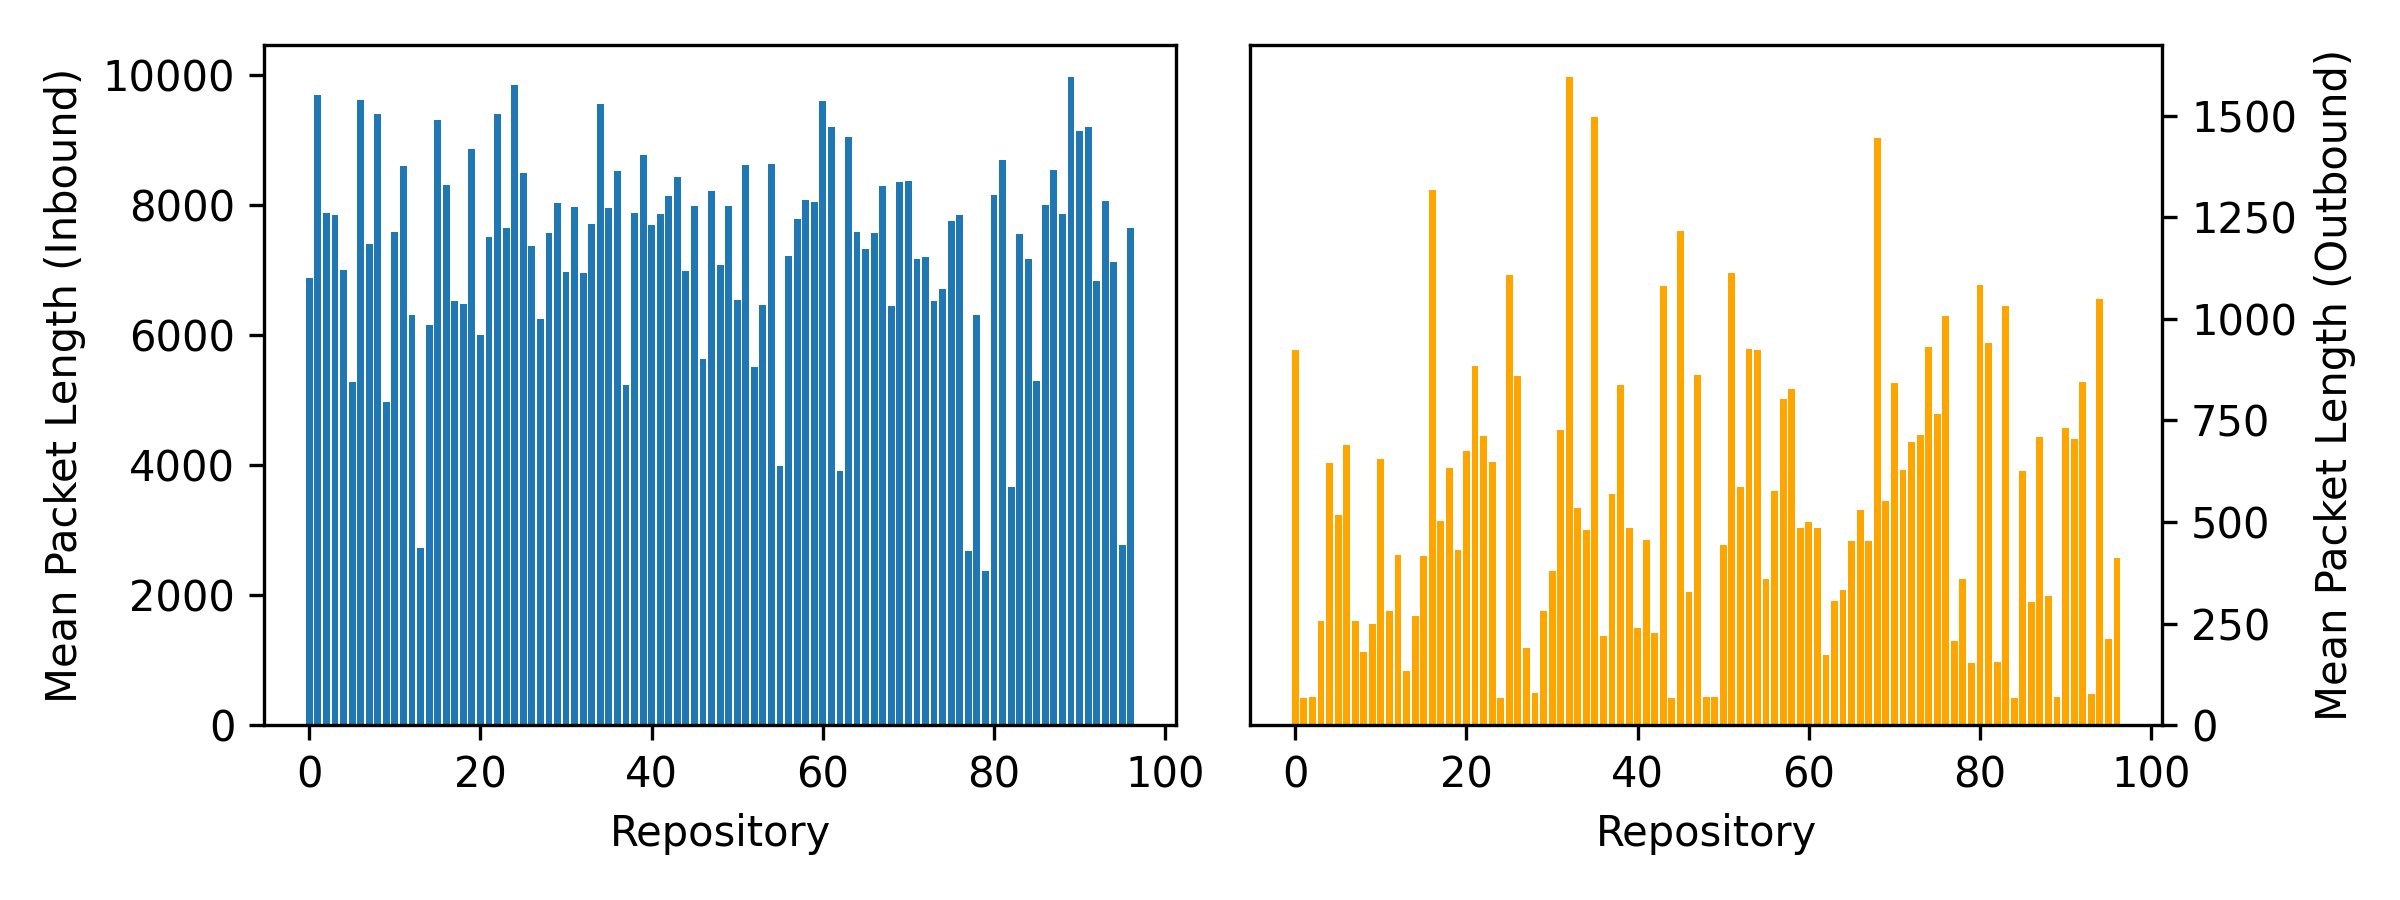
\includegraphics[width=\textwidth]{charts/mean-packet-length.png}
  \caption{Inbound and Outbound mean packet lengths across all monitored repositories over 50 clones.}
  \label{fig:packetlen}
\end{figure*}

\begin{figure*}
  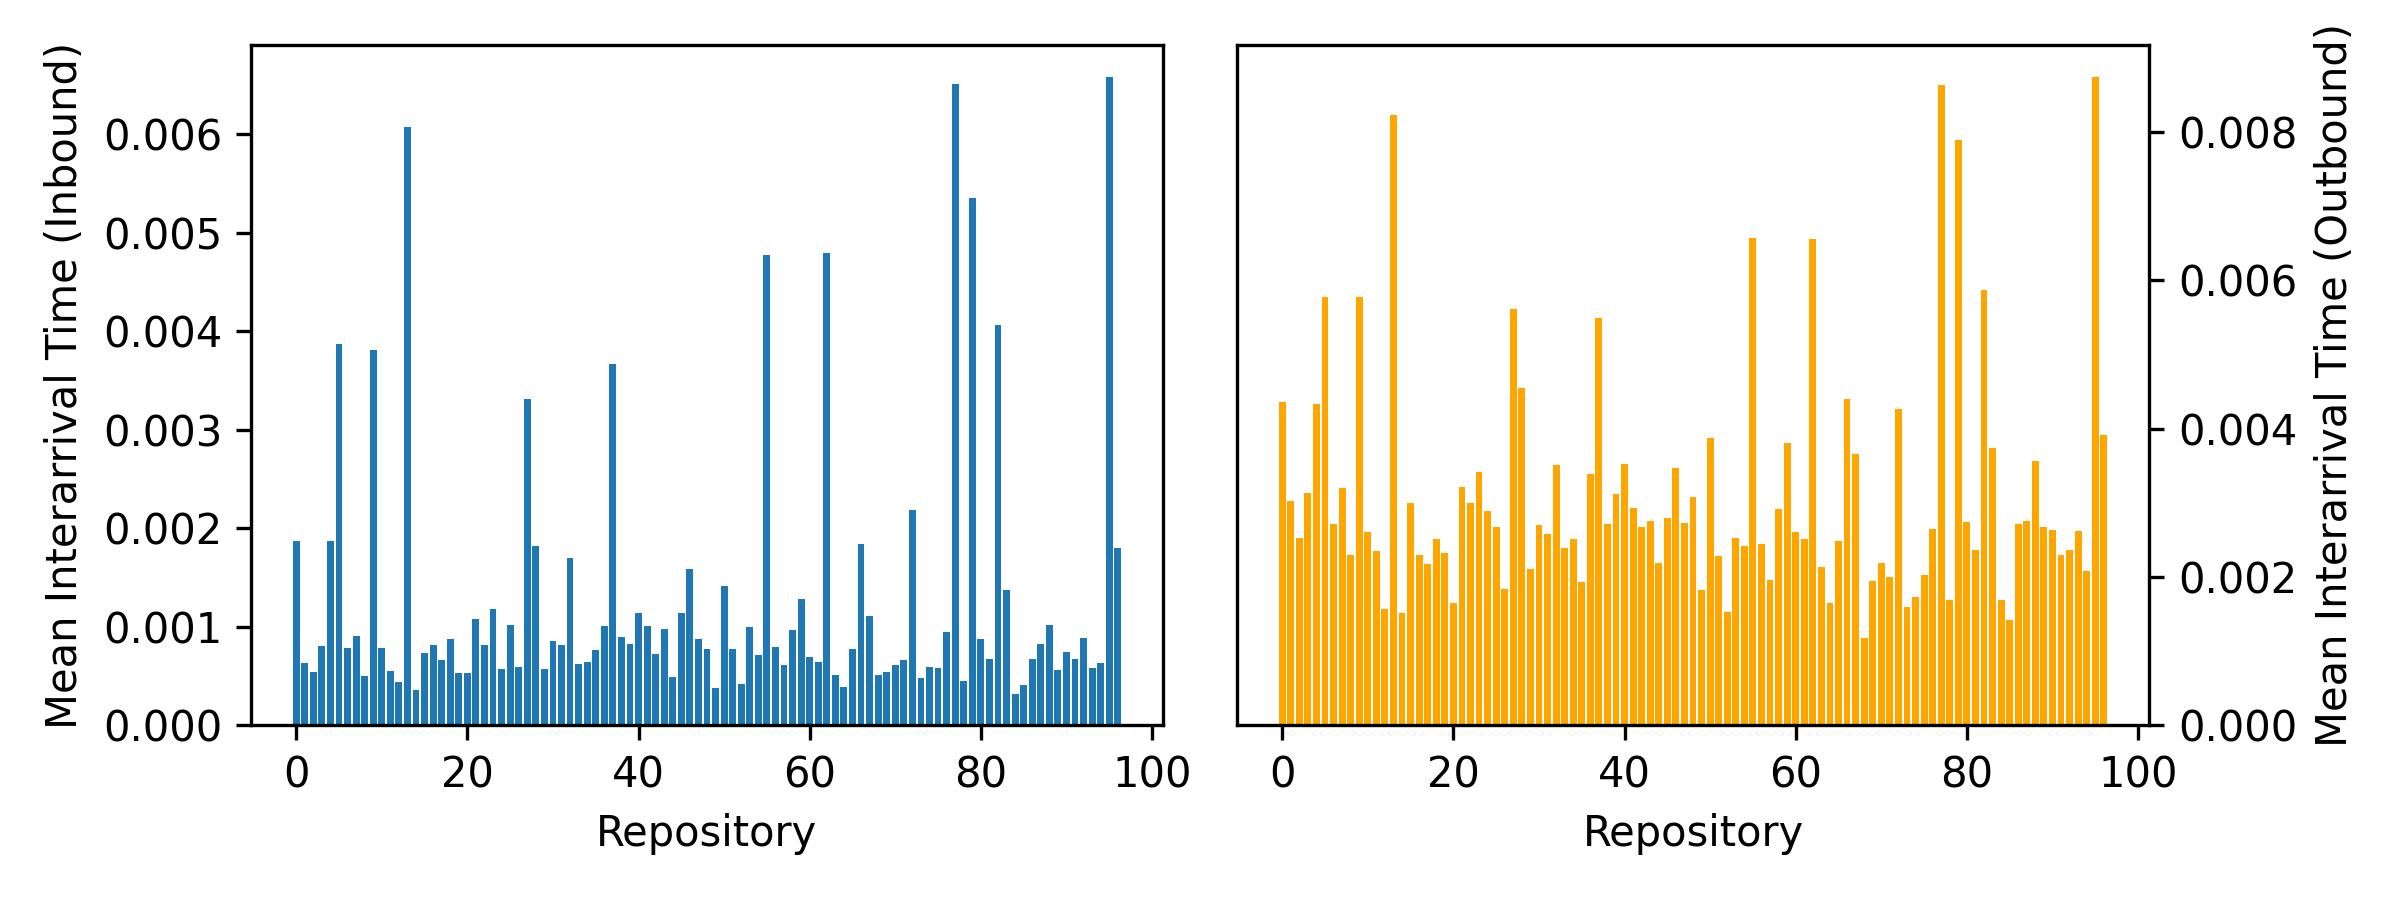
\includegraphics[width=\textwidth]{charts/interarrival-times.png}
  \caption{Inbound and Outbound mean packet interarrival times across all monitored repositories over 50 clones.}
  \label{fig:arrivaltime}
\end{figure*}

\begin{figure*}
  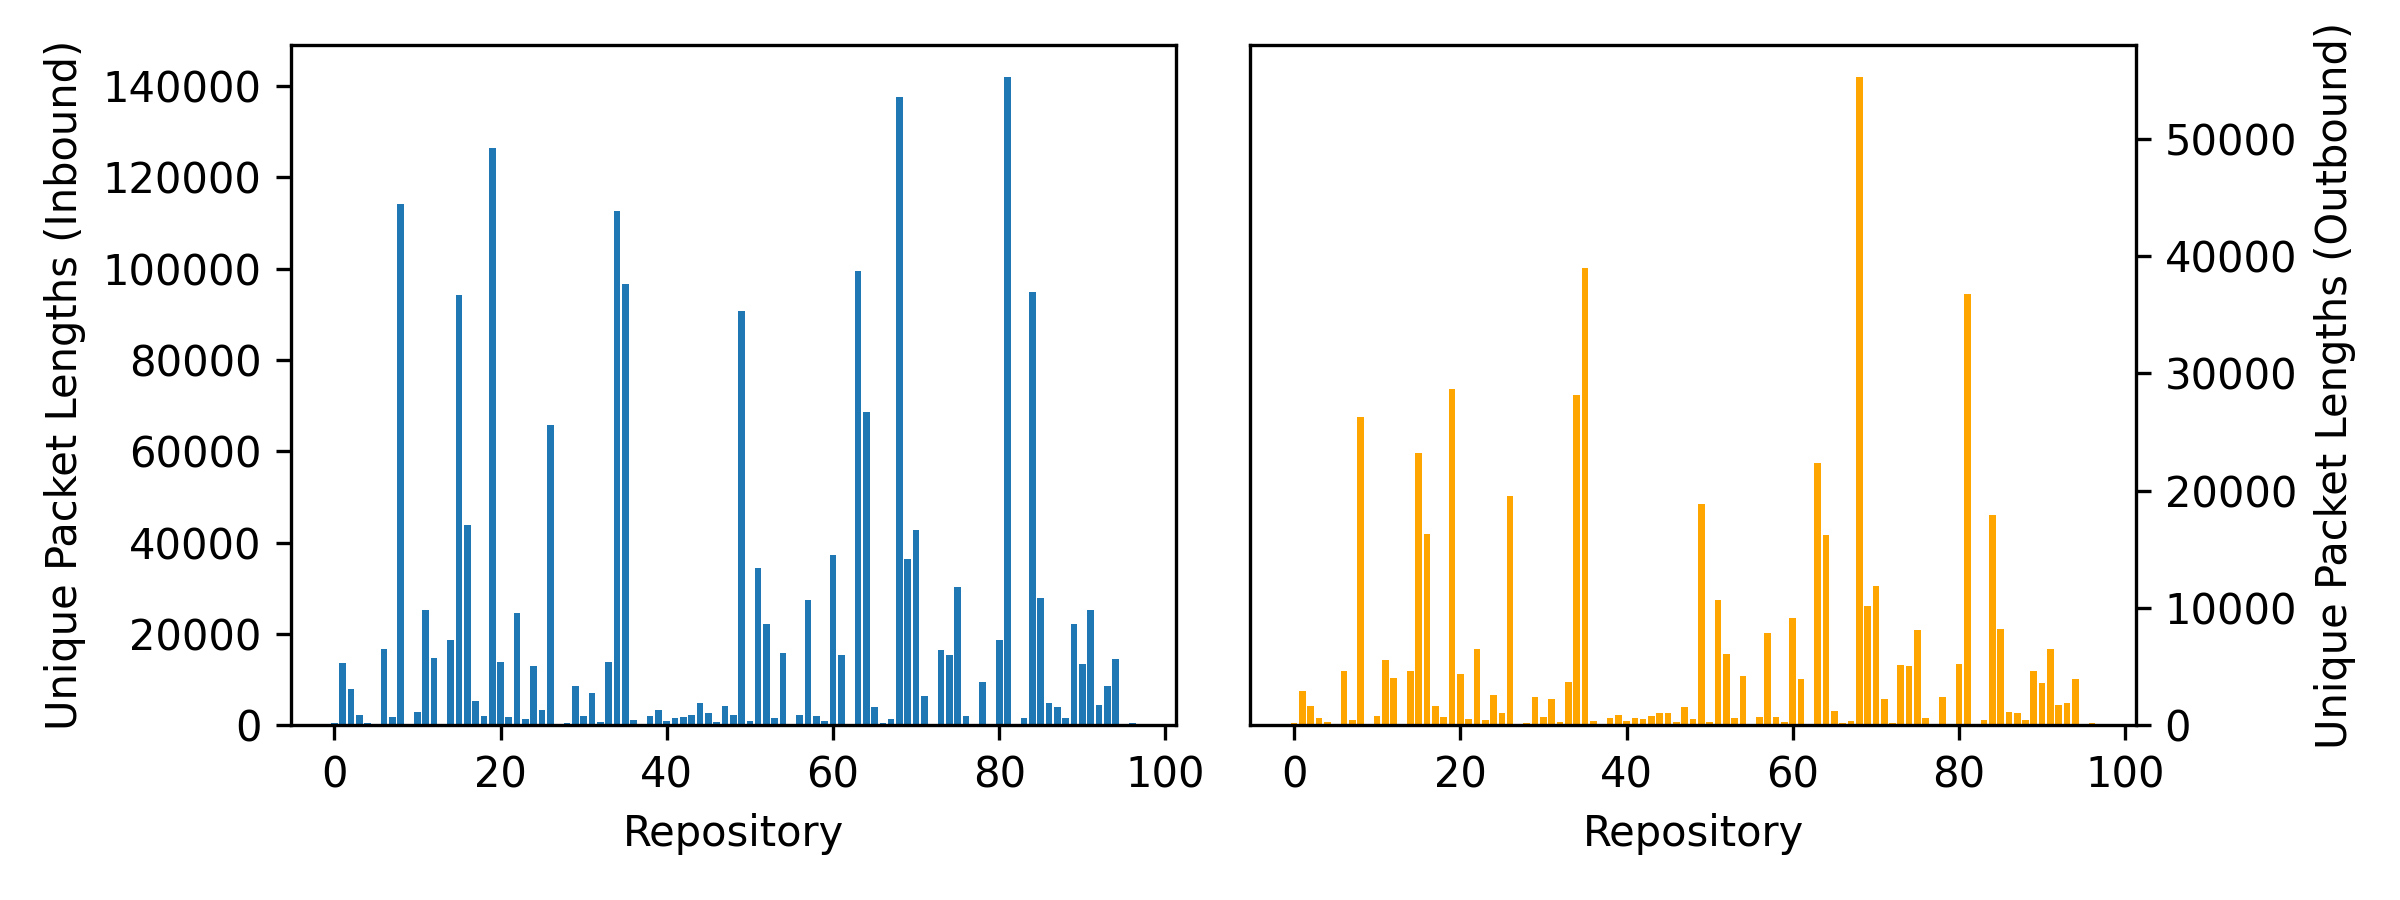
\includegraphics[width=\textwidth]{charts/unique-packet-lengths.png}
  \caption{Inbound and Outbound mean unique packet lengths across all monitored repositories over 50 clones.}
  \label{fig:uniquepacket}
\end{figure*}

\section{Results}

\subsection{Feature Distributions}
We first examined the extracted features to discern any potential patterns in the feature distributions. As seen in Figure~\ref{fig:packetlen}, inbound packet sizes were much larger than outbound packet sizes on average by nature of downloading many uncompressed files. Interestingly, the variance in outbound packet size between repositories was massive with some repositories averaging outbound packets of around \~60 bytes while other repositories averaged outbound packet lengths of \~500 bytes or greater. Further analysis is required to determine the reasoning behind this anomolic activity but we anticipate that feature distributions with higher variance, such as this one, are the ones that leak the most information in the open-world setting.

\subsection{Model Accuracy}
The feature set which achieved the best results with the Random Forest classifier was the one containing only information regarding packet length with a cross-validation accuracy of 90\%.  This was surprising because we had anticipated that more information collected would only bolster the strength of a potential adversary when performing website fingerprinting on repository traffic. Just as notable, the feature set containing exclusively time-related features was still able to achieve 49.7\% accuracy, effectively narrowing down a 96-fold classification task into a guess between 1 of 2 classes. The differences between the third and fourth feature sets seem to indicate that the three counting features for unique packet lengths have negligible impact on the final classification results.

Based on the results of our closed-world experiment alone, we were able to make some insightful observations. Our ablated featureset without regard for packet length still enabled the Random Forest classifier to achieve a cross-validation accuracy of under 50\%. This indicates that obfuscating packet lengths alone is not a viable solution to preventing a repository fingerprinting attack.

Another interesting insight is the potential for repository fingerprinting attacks to identify the contents of a private repository. Though we performed our attack against a dataset of public repositories, Github does have support for private repositories if a developer doesn't wish to share their information with the world. Though it would be impossible for a potential adversary to include a non-compromised private repository in their dataset, the presence of information leakage in repository cloning may have some implications on the notion of privacy around private repositories. The \textit{k-fingerprinting} attack, for example, attempts to link previously unseen traffic with representations learned from monitored websites. If we extend this notion to repository fingerprinting, it may be possible to identify the contents of a private repository by comparing its fingerprint with a monitored public repository.

The negligible difference in cross-validation accuracy between the second, third, and fourth feature sets call for a feature analysis specifically for packet traces scraped from repository cloning sessions. We've identified a few reasons as to why feature importance for website page loads, as described by Hayes and Danezis~\citep{hayes2016k}, may not actully be applicable when performing a website fingerprinting attack against repository cloning sessions.

The traffic patterns initiated by a repository clone operation are fundamentally different from those generated by a website pageload. With website page loads, a file containing renderable markup is served to a client's browser. This file may also contain Javascript code embedded within it to fetch additional resources from remote content distribution networks to ensure the page functions as intended for the client. 

%Write about how git clone works


\section{Conclusion}




\subsection{Potential Defenses}
%archive downloads, caveat of no commit history
%cloning with a depth of 1

\subsection{Future Work}
%feature analysis specifically for remote repo traffic

%k-fingerprinting, see if private repos can be id'ed
We've identified several directions for future work in this project. The logical next step would be to implement repository fingerprinting as an open-world k-fingerprinting attack to see how well learned features of monitored repositories can be generalized to the set of all repositories.

%deep learning classifier and discriminators



\bibliographystyle{ACM-Reference-Format}
\bibliography{sample-base}



\end{document}
\endinput
%%
%% End of file `sample-authordraft.tex'.
